\chapter{Software Architecture}
\label{ch:software-architecture}

\section{Package structure}

The repository is a pnpm workspace with four packages. Dependencies flow in one
direction only: every package may depend on \texttt{@expo-snips/core}; the core
depends on nothing from the workspace.

\begin{figure}[H]
\centering
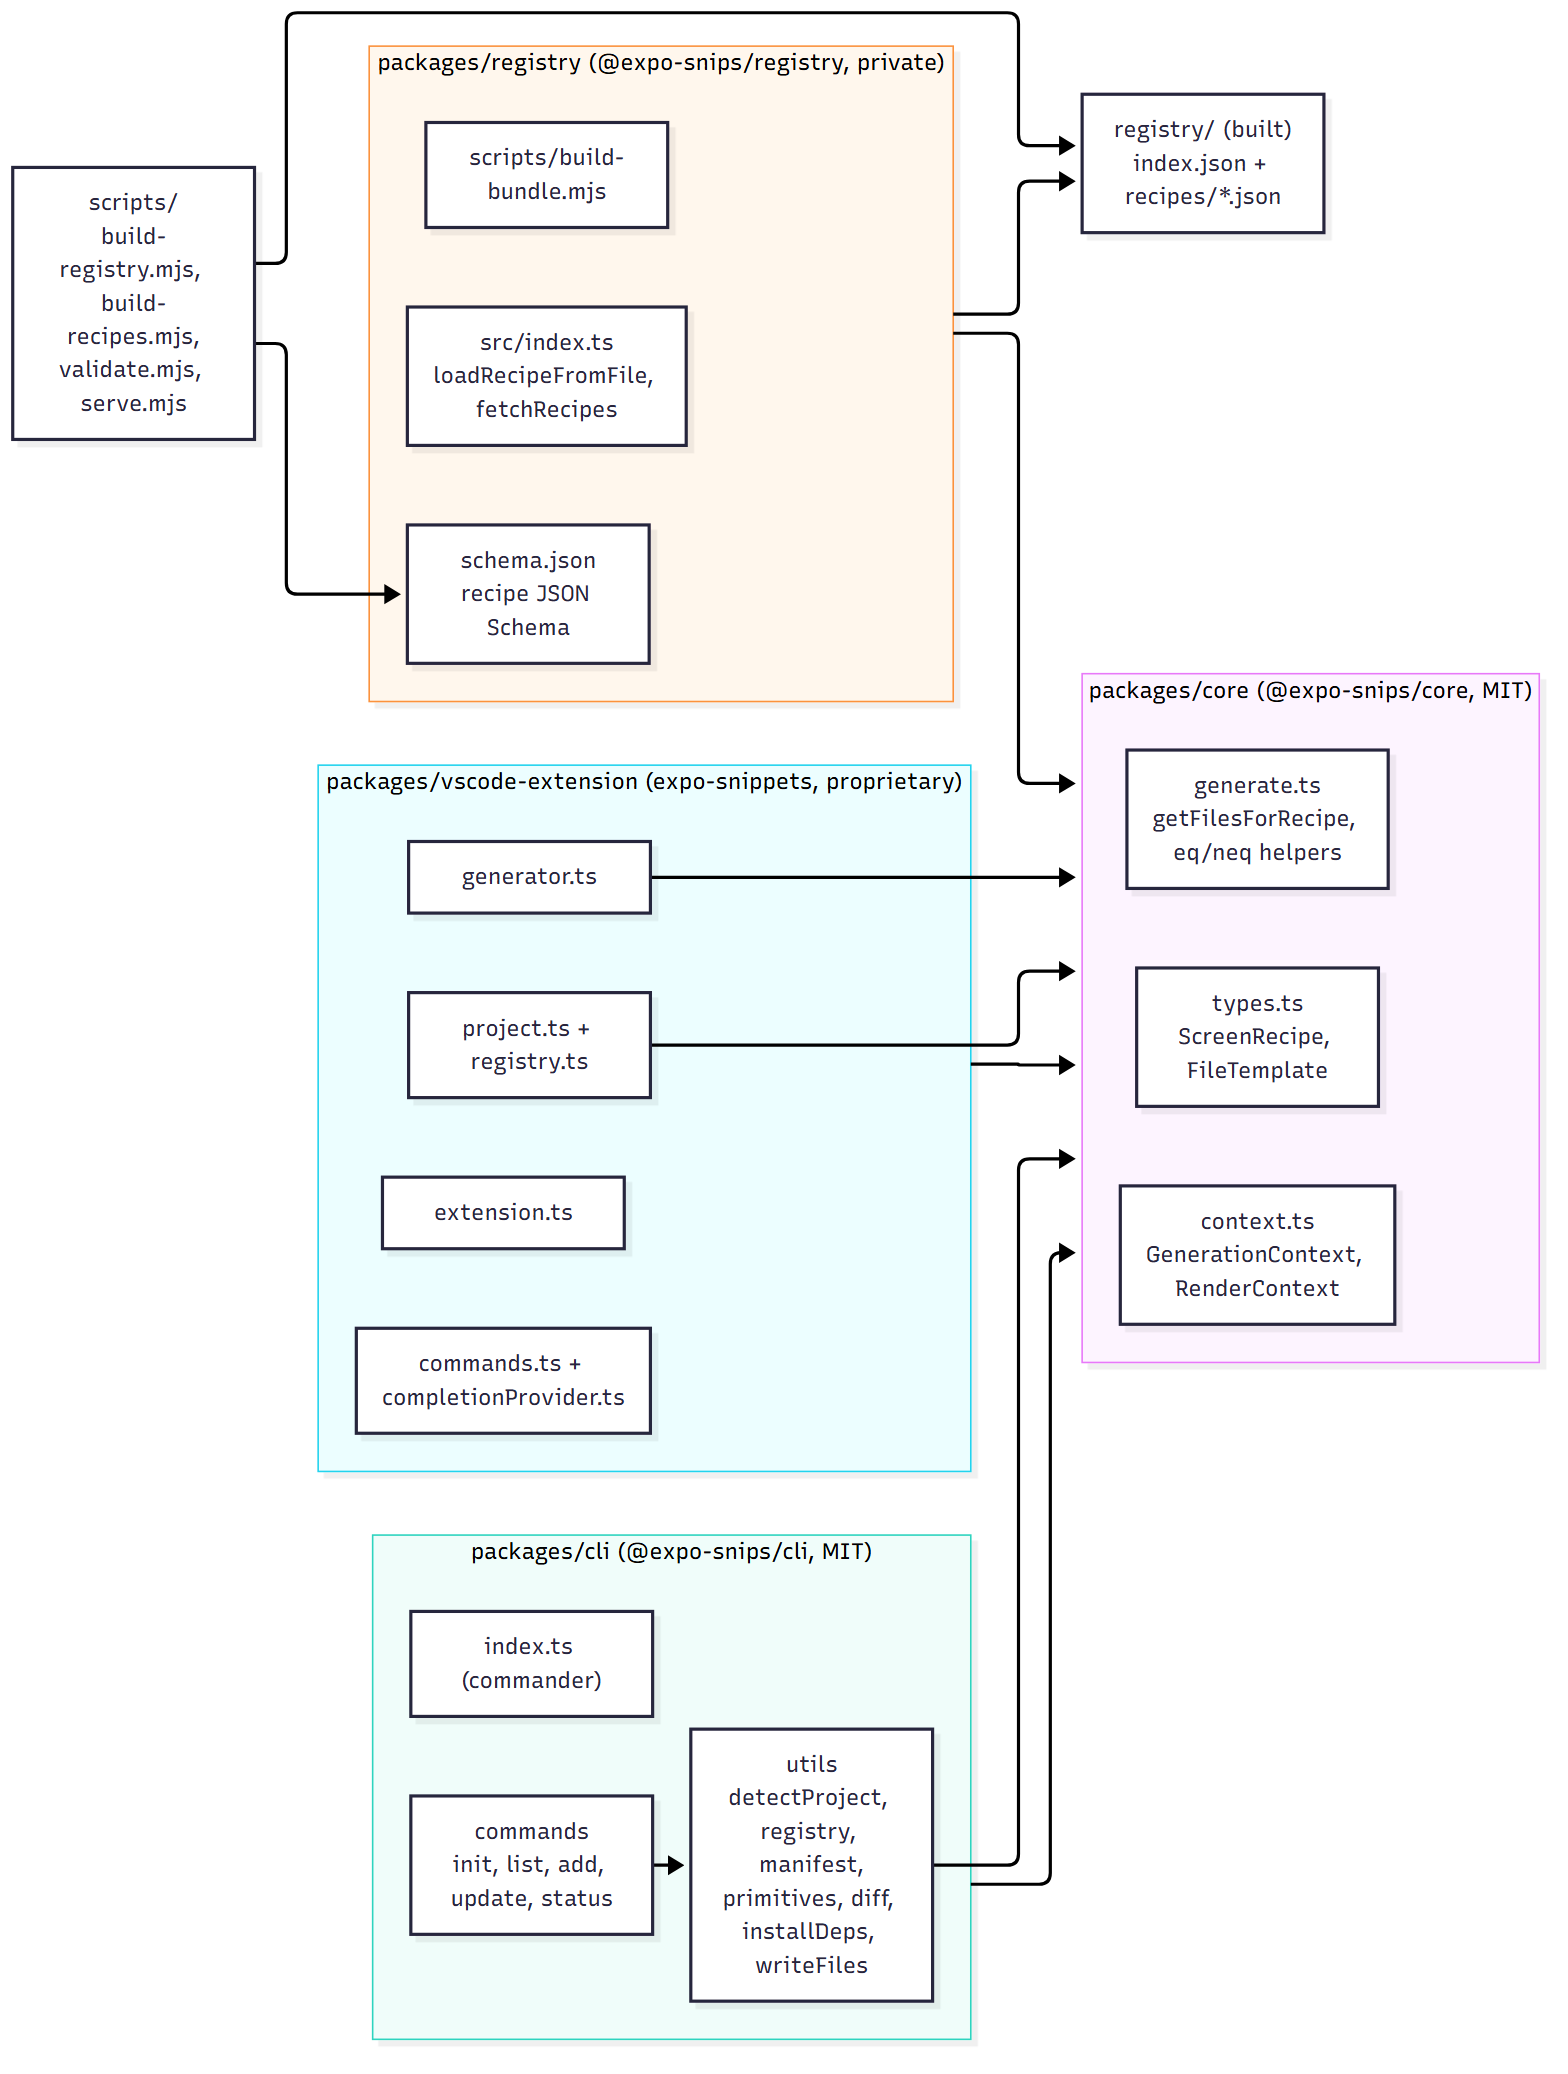
\includegraphics[width=\textwidth]{diagrams/component-architecture.png}
\caption{Component architecture of the pnpm workspace}
\label{fig:component-architecture}
\end{figure}

\begin{longtable}{@{}L{3.6cm}L{2.6cm}L{1.9cm}L{5.9cm}@{}}
\caption{Package inventory}\\
\toprule
\textbf{Package} & \textbf{Name} & \textbf{Visibility} & \textbf{Responsibility} \\
\midrule
\endfirsthead
\toprule
\textbf{Package} & \textbf{Name} & \textbf{Visibility} & \textbf{Responsibility} \\
\midrule
\endhead
\texttt{packages/core} & \texttt{@expo-snips/core} & public (MIT) & Shared types, generation context and the Handlebars rendering engine. \\
\texttt{packages/cli} & \texttt{@expo-snips/cli} & public (MIT) & Terminal client: commands, detection, orchestration, manifest, diff. \\
\texttt{packages/registry} & \texttt{@expo-snips/registry} & private & Recipe data (24), templates (48), JSON Schema, bundle builder, filesystem + HTTP loaders. \\
\texttt{packages/vscode-extension} & \texttt{expo-snippets} & proprietary & VS Code client: commands, completion, status bar, workspace detection, generation. \\
\bottomrule
\end{longtable}

Workspace dependency declarations:
\texttt{"@expo-snips/core": "workspace:*"} in \texttt{packages/cli/package.json} and
\texttt{packages/registry/package.json}; a development dependency on
\texttt{@expo-snips/core} in \texttt{packages/vscode-extension/package.json}
(the engine is bundled into the extension by esbuild).

\section{Module boundaries}

\subsection*{\texttt{@expo-snips/core}}

\begin{longtable}{@{}L{2.8cm}L{11.2cm}@{}}
\toprule
\textbf{Module} & \textbf{Contents} \\
\midrule
\endhead
\texttt{types.ts} & \texttt{StylingOption}, \texttt{RouterOption}, \texttt{UIOption},
\texttt{IconOption}, \texttt{Conditions}, \texttt{FileTemplate} (with
\texttt{perStyling} and \texttt{variants} override maps), \texttt{ScreenVariant},
\texttt{ScreenRecipe}. \\
\texttt{context.ts} & \texttt{GenerationOptions}, \texttt{GenerationContext}
(project root, options, optional variant), \texttt{RenderContext}. \\
\texttt{generate.ts} & Registers the \texttt{eq}/\texttt{neq} Handlebars helpers;
exposes \texttt{renderTemplate}, \texttt{getFilesForRecipe}; privately
\texttt{resolveTemplateString} (variant $\rightarrow$ per-styling $\rightarrow$
template precedence) and \texttt{matchesCondition}. \\
\texttt{index.ts} & Barrel re-export of the three modules above. \\
\bottomrule
\end{longtable}

The core performs no I/O and has no knowledge of the CLI, the extension or the
filesystem. This makes it the natural unit-test target, although no tests exist.

\subsection*{\texttt{@expo-snips/cli}}

\begin{longtable}{@{}L{4.2cm}L{9.8cm}@{}}
\toprule
\textbf{Module} & \textbf{Contents} \\
\midrule
\endhead
\texttt{index.ts} & Creates the \texttt{Command} program, sets name/description/version, registers the five subcommands. \\
\texttt{commands/init.ts} & Project bootstrap via \texttt{create-expo-app}; refuses when \texttt{app.json} exists. \\
\texttt{commands/list.ts} & Prints the resolved catalog with source attribution. \\
\texttt{commands/add.ts} & The main generation command: registry resolution, detection, option resolution, prompts, rendering, writing, primitives, install, manifest. \\
\texttt{commands/status.ts} & Prints manifest entries. \\
\texttt{commands/update.ts} & Re-renders tracked screens, diffs, confirms, writes, bumps versions. \\
\texttt{utils/detectProject.ts} & \texttt{detectProject(dir)} --- reads \texttt{package.json} and \texttt{tsconfig.json}. \\
\texttt{utils/registry.ts} & Registry base resolution, remote fetch with timeout, embedded-catalog fallback. \\
\texttt{utils/resolveRegistry.ts} & Wraps index resolution with user-facing source reporting. \\
\texttt{utils/manifest.ts} & Manifest read/write/upsert/version-bump. \\
\texttt{utils/primitives.ts} & Recursive primitive resolution. \\
\texttt{utils/installDeps.ts} & Package-manager detection and dependency installation. \\
\texttt{utils/writeFiles.ts} & Directory creation and file writing with per-file logging. \\
\texttt{utils/diff.ts} & LCS line diff and coloured printing. \\
\texttt{generated/registry-data.ts} & Build-time generated embedded catalog (git-ignored). \\
\bottomrule
\end{longtable}

\subsection*{\texttt{@expo-snips/registry}}

\begin{itemize}
  \item \texttt{src/index.ts} --- \texttt{loadRecipeFromFile} (inlines
        \texttt{templateFile}, variant and per-styling references),
        \texttt{getAllRecipes}, \texttt{getRecipeById}, \texttt{searchRecipes} and
        \texttt{fetchRecipes} (accepts an array, a \texttt{\{recipes\}} bundle or a
        single recipe object).
  \item \texttt{schema.json} --- the recipe JSON Schema used by the validator.
  \item \texttt{data/**} --- 24 recipe source files organised by category.
  \item \texttt{templates/**} --- 48 Handlebars templates organised by category.
  \item \texttt{scripts/build-bundle.mjs} --- writes \texttt{bundle.json} (a
        \texttt{\{version, name, recipes\}} bundle, 24 recipes).
\end{itemize}

\subsection*{\texttt{expo-snippets} (VS Code extension)}

\begin{longtable}{@{}L{4.2cm}L{9.8cm}@{}}
\toprule
\textbf{Module} & \textbf{Contents} \\
\midrule
\endhead
\texttt{extension.ts} & \texttt{activate()}: registers commands and completion
provider, creates the status bar item; \texttt{deactivate()} is empty. \\
\texttt{commands.ts} & \texttt{expo-snips.addScreen} (Quick Pick) and
\texttt{expo-snips.generateFromCompletion}. \\
\texttt{completionProvider.ts} & Completion provider for the four TS/JS language
ids, triggered on \texttt{:}, matching \texttt{snip:} / \texttt{expo-snips:}. \\
\texttt{generator.ts} & \texttt{resolveOptions}, \texttt{pickVariant},
\texttt{detectPackageManager}, \texttt{installDependencies},
\texttt{resolvePrimitives}/\texttt{getPrimitives} and \texttt{generateScreen}. \\
\texttt{project.ts} & \texttt{getWorkspaceRoot}, \texttt{detectProject} and the
manifest functions. \\
\texttt{registry.ts} & Embedded catalog, remote index/recipe fetch, 5-minute cache
and back-off. \\
\bottomrule
\end{longtable}

\section{Dependency graph}

\begin{table}[H]
\centering
\caption{Runtime and build dependencies}
\begin{longtable}{@{}L{3.6cm}L{4.6cm}L{5.8cm}@{}}
\toprule
\textbf{Package} & \textbf{Runtime dependencies} & \textbf{Dev / build dependencies} \\
\midrule
\endhead
core & handlebars \^{}4.7.8 & typescript \^{}5.5 \\
cli & @expo-snips/core (workspace), chalk \^{}4.1.2, commander \^{}12, fs-extra \^{}11.2, prompts \^{}2.4.2 & @types/fs-extra, @types/node \^{}20, @types/prompts, typescript \^{}5.5 \\
registry & @expo-snips/core (workspace) & @types/node \^{}20, typescript \^{}5.5 \\
vscode-extension & (none at runtime; engine bundled) & @expo-snips/core, @types/fs-extra, @types/node \^{}20, @types/vscode \^{}1.80, @vscode/vsce \^{}2.24, esbuild \^{}0.21.5, fs-extra \^{}11.2, typescript \^{}5.5 \\
\bottomrule
\end{longtable}
\end{table}

\section{Build pipeline}

\begin{longtable}{@{}L{4cm}L{10cm}@{}}
\toprule
\textbf{Package} & \textbf{Build command and behaviour} \\
\midrule
\endhead
core & \texttt{tsc -p tsconfig.json} --- emits \texttt{dist/} with declarations and source maps. \\
cli & \texttt{node scripts/prepare-registry.mjs \&\& tsc -p tsconfig.json} --- regenerates the embedded catalog, then compiles. \\
registry & \texttt{tsc} (library build) and \texttt{node scripts/build-bundle.mjs} (\texttt{build:bundle}). \\
vscode-extension & \texttt{node esbuild.mjs} --- runs \texttt{prepareRegistry()} first, then bundles to \texttt{out/extension.js}. \\
root & \texttt{pnpm -r build}; also \texttt{validate}, \texttt{build:registry} and \texttt{serve} scripts. \\
\bottomrule
\end{longtable}

\section{Code-size profile}

The hand-written TypeScript across the workspace (excluding type declarations and
generated catalog modules) is approximately 1{,}600 lines. The largest single
source files are \texttt{generator.ts} (268 lines), \texttt{add.ts} (279 lines) and
\texttt{update.ts} (150 lines). No file is pathological in size; the largest
codebase element by far is the recipe data and template set (24 recipes and 48
templates).

\textbf{Status:} IMPLEMENTED (measured) / INFERRED (assessment that no file is
pathological).
